\subsubsection{\large{Хранилище расчётных данных}}
\addcontentsline{toc}{subsubsection}

Детальная архитектура хранилища расчётных данных представлена на диаграмме компонент
(см. рис\ \ref{pic:architecture__storage-component}).

\begin{figure}[H]
	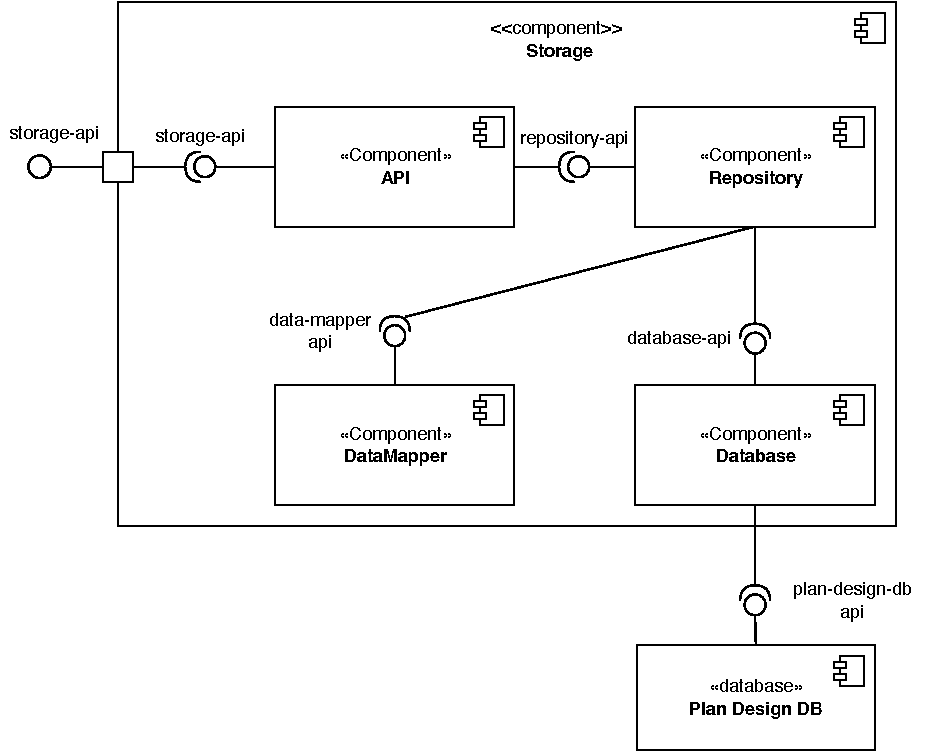
\includegraphics[width=\textwidth]{architecture/pictures/storage/component_common}
	\caption{Диаграмма компонент хранилища расчётных данных}
	\label{pic:architecture__storage-component}
\end{figure}
\vskip 5 mm

Сервис представлен следующими компонентами:
\begin{enumerate}
	\item {
		\textit{API} -- отвечает за предоставление REST API.
	}
	\item {
		\textit{Repository} -- отвечает за получение и сохранение данных, а также логику их преобразований.
	}
	\item {
		\textit{EntityDataMapper} -- преобразование сущностей базы данных в сущности расчётной модели данных.
	}
	\item {
		\textit{Database} -- чтение/сохранение сущностей базы данных.
	}
\end{enumerate}